\section{Theorie}
\label{sec:Theorie}
Der Compton-Effekt beschreibt die Vergrößerung der Wellenlänge von $\gamma$-Strahlung bei Streuung an einem Elektron.
Um die Compton-Wellenlänge zu bestimmen wird Röntgenstrahlung an einem Plexiglasquader gestreut und das Transmissionsverhalten beobachtet.
Trifft Röntgenstrahlung auf Materie, so kann zum einen die kohärente Streuung / inelastische Streuung beobachtet werden und zum anderen die frequenzverschobene inkohärente Streuung (elastisch).
Bei Ersteres trifft das Photon auf ein freies Elektron und gibt einen Teil seiner Energie ab und wird dabei um den Winkel $\theta$ gestreut. 
Mithilfe der Energie- und Impulserhaltung folgt für die Wellenlängendifferenz $\Delta \lambda$
\begin{equation*}
    \Delta \lambda = \lambda_2 - \lambda_1
\end{equation*}
\begin{equation}
    \Delta \lambda = \frac{h}{m_e c} (1 - \cos \theta) .
    \label{eqn:lam}
\end{equation}
Dabei beschreibt $\lambda_1$ die Wellenlänge des einfallenden Photons, $\lambda_2$ die verschobene Wellenlänge des gestreuten Photons und $\theta$ den gestreuten Winkel.
\\
Die Compton-Wellenlänge ist eine Konstante und wird nach
\begin{equation}
    \lambda_c = \frac{h}{m c}
\end{equation}
bestimmt.
Die Wellenlängenverschiebung wird für $\theta = \SI{0}{\degree}$ minimal und für $\theta = \SI{180}{\degree}$ maximal (siehe \autoref{eqn:lam}).
\\
Um Röntgenstrahlung zu erzeugen wird mithilfe einer Glühkathode Elektronen emittiert und auf eine Anode hin beschleunigt.
Treffen die Elektronen auf die Anode entsteht Röntgenstrahlung.
Das Elektron wird im Coulombfeld des Atoms gebremst (Bremsspektrum).
Dabei wird ein Photon abgegeben, dessen Energie der des Elektrons abgegebenen Energie entspricht.
\\
Das charakteristische Spektrum beschreibt wie ein Elektron aus der äußeren Schale durch die Ionisierung des Anodenmaterials in die innere Schale springt.
Bei diesem Prozess wird ein Photon abgegeben, dessen Energie die Energiedifferenz der beiden Atomschalen entspricht.
Das charakteristische Spektrum besteht daher aus scharfen Linien, dessen Energie abhängig von dem Anodenmaterial ist.
Um die Compton-Wellenlänge zu bestimmen, wird die Absorption und Transmission von Röntgenstrahlung durch Aluminum untersucht.
\\
Die Intensität nach der Absorption von Photonen berechnet sich nach dem Delamber'schen Gesetz
\begin{equation}
    I = I_0 e^{-\mu d} .
\end{equation}
$I_0$ bezeichnet die auf die Aluminiumplatte mit der Dicke $d$ einfallende Intensität.
Der Absorptionskoeffizient $\mu$ hängt von der Paarbildung, dem Photoeffekt und dem Comptoneffekt ab.
\\
Mithilfe der Bragg'schen Reflexion 
\begin{equation}
    2 d \sin \alpha = n \lambda
    \label{eqn:lambdaalpha}
\end{equation}
kann die Wellenlänge $\lambda$ bei bestimmter Beugungsordnung $n$ bestimmt werden.
\begin{figure}
    \centering
    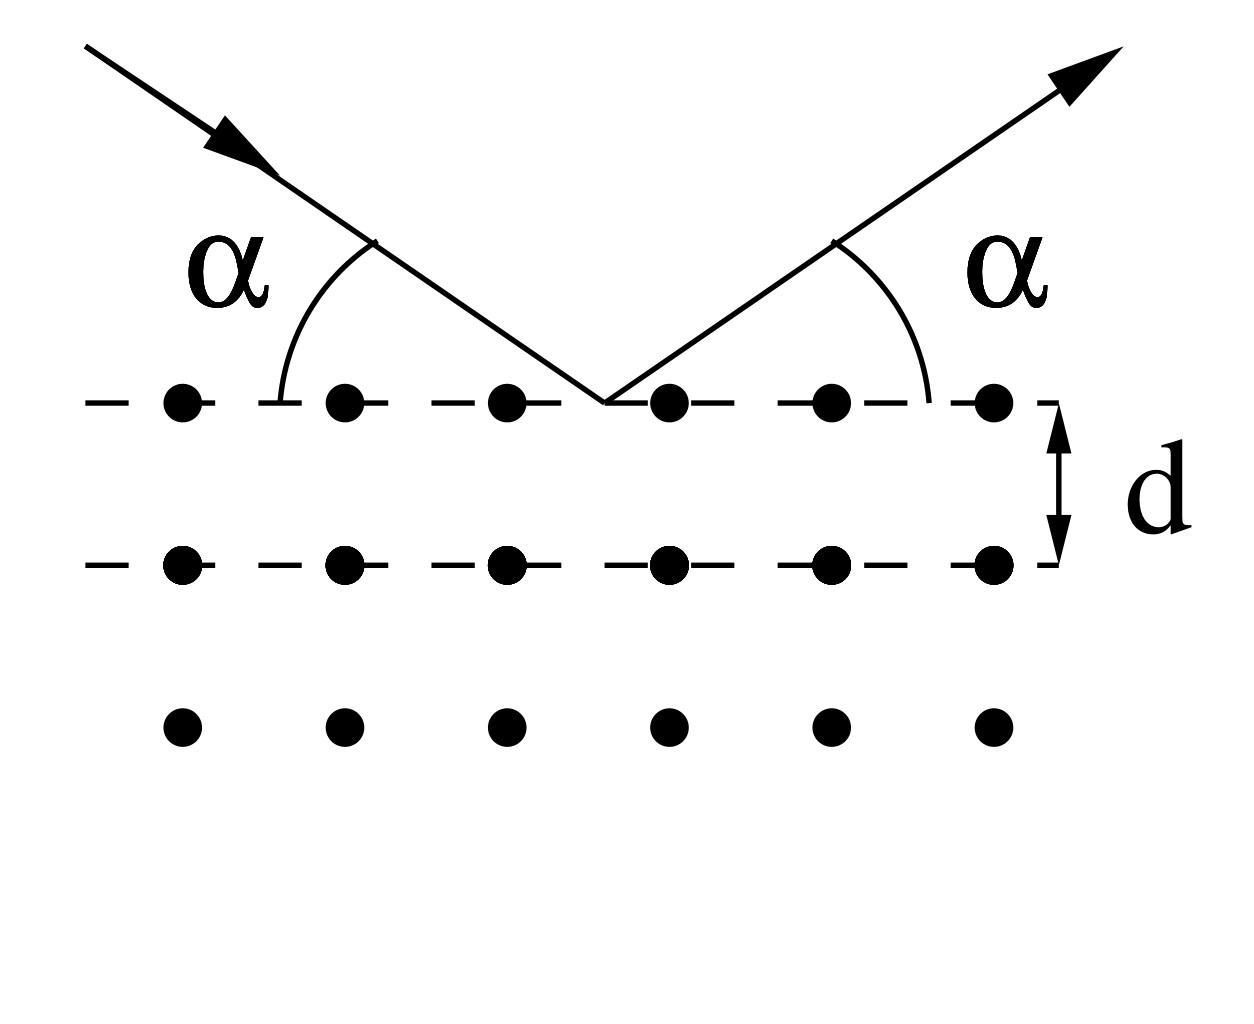
\includegraphics[width=0.3\textwidth]{content/data/kristall.jpg}
    \caption{Bragg'sche Reflexion graphisch dargestellt. \cite[2]{anleitung}}
    \label{fig:bragg}
\end{figure}
Fällt Röntgenlicht auf ein 3D-Gitter, so werden die Photonen an jedem Atom des Gitters gebeugt (siehe Abb. \ref{fig:bragg}).
Bei einem bestimmten Winkel $\alpha$, werden die Wellen perfekt überlagert (konstruktive Interferenz).
Die Gitterkonstante kann hier als $d_\text{LiF}=\SI{201.4}{\pico\metre}$ angenommen werden.